\section{Implementation in the \tnreason package}\label{cha:implementation}

We here document the implementation of the discussed concepts in the \python package \tnreason.
 
 % Name
\tnreason is an abbreviation of \textbf{t}ensor \textbf{n}etwork \textbf{reason}ing, by which we emphasize the capabilities of this package to represent and answer reasoning tasks by tensor network contractions. 

% Installation
The package can be installed either by cloning \href{https://github.com/EnexaProject/enexa-tensor-reasoning}{https://github.com/EnexaProject/enexa-tensor-reasoning} or by
\begin{centeredcode}
	!pip install tnreason
\end{centeredcode}


\subsection{Script Language}\label{subsec:scriptLanguage} % To encoding?

To specify propositional sentences, neuro-symbolic architectures and Markov Logic Networks, we developed a script language.

\subsubsection{Propositional Sentences by Nested Lists}

%\textbf{Production Rules}
Are those of Propositional Logics, but instead of brackets we nest the symbols into lists.

% Connectives
\textbf{Connectives} are represented by strings, where the following are supported (see Definition~\ref{def:connectives}):
\begin{center}
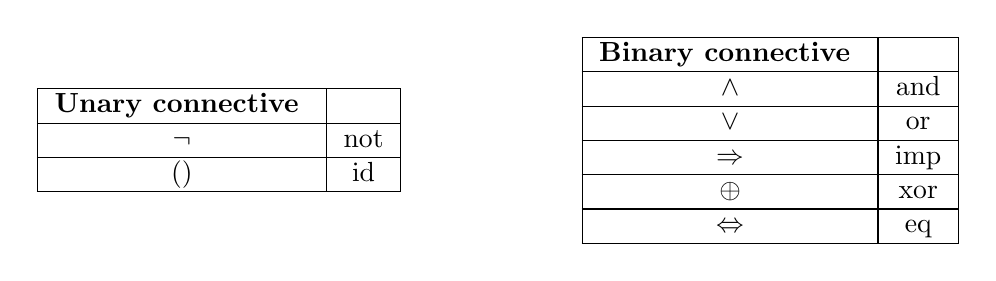
\begin{tikzpicture}
\node [anchor=center] at (0,0) {
	\begin{tabular}{|c|c|}
  	\hline
 	\textbf{Unary connective $\exconnective$} & \textbf{$\synencodingof{\exconnective}$} \\
  	\hline
 	$\lnot$ 	&  \stringof{not} \\
  	\hline
 	$()$		&  \stringof{id} \\
  	\hline
	\end{tabular}};
\node [anchor=center] at (7,0) {
	\begin{tabular}{|c|c|}
  	\hline
 	\textbf{Binary connective $\exconnective$} & \textbf{$\synencodingof{\exconnective}$} \\
  	\hline
 	$\land$ 		&  \stringof{and} \\
  	\hline
 	$\lor$ 		&  \stringof{or} \\
  	\hline
 	$\Rightarrow$ 	&  \stringof{imp} \\
  	\hline
	 $\oplus$ 		&  \stringof{xor} \\
  	\hline
	 $\Leftrightarrow$ &  \stringof{eq} \\
  	\hline
	\end{tabular}};
\end{tikzpicture}
\end{center}

% Atoms
\textbf{Atomic Formulas} are represented by arbitrary strings, which are not used for the representation of connectives. 
We further avoid the symbols \{\stringof{(}, \stringof{)}, \stringof{\_}\} in the names of atoms, to not confuse them with colors of categorical variables.

% Composed Formulas
\textbf{Composed Formulas} $\exformula_1\exconnective,\exformula_2$ are represented by 
\begin{centeredcode}
	[$\synencodingof{\exconnective}$, $\synencodingof{\exformula_1}$, $\synencodingof{\exformula_2}$]
\end{centeredcode}
where we apply the conventions
\begin{itemize}
	\item Connectives are at the 0th position in each list
	\item Further entries are either atoms as strings or encoded formulas itself
\end{itemize}

% Backus-Naur
The applied grammar in Backus-Naur form is \\
\begin{tabular}{|l|l|}
  	\hline
 	Unary Connective & \stringof{not} | \stringof{id}\\
  	\hline
 	Binary Connective & \stringof{and} | \stringof{or} | \stringof{imp} | \stringof{xor}  | \stringof{eq} \\ 
  	\hline
 	Atomic Formula & Set of strings not in Connectives\\
  	\hline
	Complex Formula & Atomic Formula | [Unary Connective, Complex Formula] | \\
	&  [Binary Connective, Complex Formula, Complex Formula] \\
	\hline
\end{tabular}


\begin{example}[Encoding of the Wet Street example]
For example we have
\begin{itemize}
	\item 
	Atomic variable $\var{Rained}$ by
		\begin{centeredcode}
			$\synencodingof{\var{Rained}}$ 
			= \stringof{Rained}
		\end{centeredcode}
	\item 
	Negative literal $\lnot\var{Rained}$ by
		\begin{centeredcode}
			$\synencodingof{\lnot\var{Rained}}$ 
			= [\stringof{not},\stringof{Rained}]
		\end{centeredcode}
	\item 
	Horn clause $\left(\var{Rained}\Rightarrow\var{Wet}\right)$ by 
 		\begin{centeredcode}
			$\synencodingof{\var{Rained}\Rightarrow\var{Wet}}$ 
			= [\stringof{imp},\stringof{Rained},\stringof{Wet}]
		\end{centeredcode}
	\item 
	Knowledge Base
	$(\lnot\var{Rained})\land(\var{Rained}\Rightarrow\var{Wet})$ by
		\begin{centeredcode}
			$\synencodingof{\lnot\var{Rained})\land(\var{Rained}\Rightarrow\var{Wet}}$ 
			=  [\stringof{and}, [\stringof{not}, \stringof{Rained}], [\stringof{imp}, \stringof{Rained}, \stringof{Wet}]]
		\end{centeredcode}
\end{itemize}
\end{example}




\subsubsection{Knowledge Bases}

% Should distinguish these in knowledge?
We distinguish here formulas, with propositional logic interpretation and formulas which have a soft logic interpretation.
%\textbf{Facts.} 
The formulas with hard interpretation are called facts in a knowledge base $\kb$ and encoded by dictionaries
\begin{centeredcode}
	\{key($\exformula$) : $\synencodingof{\exformula}$ for $\exformula\in\kb$ \}
\end{centeredcode}

\subsubsection{Markov Logic Networks}

%\textbf{Weighted formulas.} 
The formulas with soft interpretation are called weighted formulas and encoded by $\expof{\weightof{\exformula}\cdot\exformula}$.
We thus require a specification of the weights, which we do by adding $\weightof{\exformula}$ as a $\mathrm{float}$ or an $\mathrm{int}$ to the list $\synencodingof{\exformula}$.
We then store Markov Logic Networks by dictionaries
\begin{centeredcode}
	\{key($\exformula$) : $\synencodingof{\exformula}$ + [$\weightof{\exformula}$] for $\exformula\in\formulaset$\}
\end{centeredcode}

\subsubsection{Neuro-Symbolic Architecture by Nested Lists}

% Generalizing the script language to specify architectures
To specify neuro-symbolic architectures in terms of formula selecting maps, as has been the subject of Chapter~\ref{cha:architectures} we further exploit the nested list structure of encoding propositional logics.
We replace, in each hierarchy of the nested structure each entry by a list of possible choices.
In this way, we reinterpret the list index as the choice indices $\parindex$ introduced for connective and formula selections (see Definition~\ref{def:connectiveSelector} and \ref{def:formulaSelector}).

% Neurons
A connective selector (see Definition~\ref{def:connectiveSelector}) is encoded by the list
	\begin{centeredcode}
			$\synencodingof{\exconnective}$ 
			= [$\synencodingof{\exconnective_{0}}$, $\ldots$, $\synencodingof{\exconnective_{\parlegdim\shortminus1}}$]
	\end{centeredcode}
and a formula selector (see Definition~\ref{def:formulaSelector}) by
	\begin{centeredcode}
			$\synencodingof{\fselectionmap}$ 
			= [$\synencodingof{\exconnective_{0}}$, $\ldots$, $\synencodingof{\exconnective_{\parlegdim\shortminus1}}$]
	\end{centeredcode}
A logical neuron of order $\parorder$ (see Definition~\ref{def:fsNeuron}), defined by a connective selector $\exconnective$, and a formula selector $\fselectionmap_\atomenumerator$ on each argument $\atomenumerator\in[\parorder]$, is encoded by
		\begin{centeredcode}
			$\synencodingof{\lneuron}$ 
			= [$\synencodingof{\exconnective}$, $\synencodingof{\fselectionmap_0}$, $\ldots$,  $\synencodingof{\fselectionmap_{\parorder-1}}$]
		\end{centeredcode}
Only the unary $\parorder=1$ and the $\parorder=2$ cases are supported.


% Confusing?
The resulting nested lists indices have an alternating interpretation at each level compared with the elements of each list.
That is, when $\synencodingof{\lneuron}$ is the encoding of a neuron, then any element $x\in\synencodingof{\lneuron}$ represents a list of choices.
When $x$ is not the first element, then each choice is either the encoding $\synencodingof{\catvariable}$ of an atomic formula, or another neuron. 

% Find another symbol?
A neural architecture $\larchitecture$ is then represented in the dictionary
\begin{centeredcode}
	$\synencodingof{\larchitecture}$ = \{key($\lneuron$) : $\synencodingof{\lneuron}$ for $\exformula\in\larchitecture$\}
\end{centeredcode}
%To store this structure, we choose dictionaries of neuron spe
%\begin{centeredcode}
%	\{key($\lneuron$) : $\synencodingof{\lneuron}$ for $\exformula\in\formulaset$\}
%\end{centeredcode}
where key($\lneuron$) is a string, which can be used in the formula selections of other neurons.

% Important for well-definedness
It is important that the directed graph of neurons induced by the choice possibilities is acyclic, to ensure well-definedness of the architecture.


% Backus-Naur
In order to represent neuro-symbolic architectures, the grammar of $\synencodingof{\cdot}$ in Backus-Naur Form is extended by the production rules \\
\begin{tabular}{|l|l|}
  	\hline
 	Unary Connectives & [Unary Connective] | [Unary Connective] + Unary Connectives \\
  	\hline
 	Binary Connectives & [Unary Connective] | [Binary Connective] + Binary Connectives \\
	%\hline
	%Neuron Name & Any set of strings not used for atoms or connectives \\
  	\hline
 	Dependency Choice & Atomic Formula | Neuron \\ 
  	\hline
	Dependency Choices & [Dependency Choice] | [Dependency Choice] + Dependency Choices \\ 
	\hline
	Neuron & [Unary Connectives, Dependency Choices] | \\
	&  [Binary Connectives, Dependency Choices, Dependency Choices] \\
	\hline
\end{tabular}


\begin{example}[Neuro-Symbolic Architecture for the Wet Street]
	Following the wet street example, we can define a neuron by
	\begin{centeredcode}
		$\synencodingof{\lneuron}$ = [[\stringof{imp},\stringof{eq}],[\stringof{Wet},\stringof{Sprinkler}],[\stringof{Street}]] 
	\end{centeredcode}
	from which the formulas 
	\begin{centeredcode}
		[\stringof{imp}, \stringof{Wet}, \stringof{Street}] \\
		\hspace{0.25cm} [\stringof{eq}, \stringof{Wet}, \stringof{Street}] \\
		\hspace{1cm}[\stringof{imp}, \stringof{Sprinkler}, \stringof{Street}] \\
		\hspace{1cm}[\stringof{eq}, \stringof{Sprinkler}, \stringof{Street}]		
	\end{centeredcode}
	can be chosen.
	Combining this neuron with further neurons, e.g. by the architecture
	\begin{centeredcode}
		$\synencodingof{\larchitecture}$ = \{ \stringof{neur1}: [[\stringof{imp},\stringof{eq}],[\stringof{neur2}],[\stringof{Street}]] , \\
		\hspace{1.8cm}\stringof{neur2}: [[\stringof{lnot},\stringof{id}],[\stringof{Wet},\stringof{Sprinkler}],[\stringof{Street}]] \}
	\end{centeredcode}
	the expressitivity increases.
	In this case, the further neuron provides the flexibility of the first atoms to be replaced by its negation.	
\end{example}



\subsection{Tensor Networks} % -> To engine section?

\subsubsection{Core Nomenclature}

% See in encoding subpackage
Appearing cores:
\begin{itemize}
	\item "\_conCore": logical connectives (relational encoding of the connective map)
	\item "\_headCore": Binary vectors representing of the exponential (directly a tensor)
	\item "\_dataCore": Representing (relational encoding of the data map)
\end{itemize}

\subsubsection{Color Nomenclature}

Represent the three appearing types of variables:
\begin{itemize}
	\item Categorical variables $\catvariableof{\cdot}$: cVar / aVar
	\item Selection variables $\selvariableof{\cdot}$: sVar % differing suffixes actVar, selVar! -> unify them
	\item Term variables $\indvariableof{\cdot}$: tVar % so far without suffix, just atom names, toDo: tVar
\end{itemize}




\subsection{Contraction Calculus} % -> To engine section?

We have described two main encoding schemes of functions, by a direct interpretation of functions as tensors or a more relational encoding.
Both come with a different calculus scheme, which we have framed coordiante calculus and basis calculus.

\subsubsection{Coordinate Calculus}

Main function
\begin{centeredcode}
	engine.coordinate\_transform(coresList, transformFunction)
\end{centeredcode}

\subsubsection{Basis Calculus}

Main function 
\begin{centeredcode}
	engine.relational\_encoding()
\end{centeredcode}
basis calculus then based on contractions




\subsection{Architecture}

\tnreason is structured in four subpackages and three layers
\begin{itemize}
	\item Layer 1: Storage and numerical manipulations, by subpackage \spengine, "Tensor Networks" -> building "tn" of \tnreason
	\item Layer 2: Specification of workload, subpackage \spencoding specific for storage, subpackage \spalgorithms specific for manipulations
	\item Layer 3: Applications in reasoning, by subpackage \spknowledge, "Reasoning" -> building "reason" of \tnreason
\end{itemize}

We sketch this structure by
\begin{center}
\begin{tikzpicture}[scale=0.35]

\draw[dashed] (-30,15) -- (12,15) -- (12,-3) -- (-30,-3) -- (-30,15);

\draw (-10,10) rectangle (10,14); 
\node [anchor=center] at (0,12) {\spknowledge};

\node [anchor=center] at (-20,12) {\layerthreespec};
\draw[dashed] (-30,9) -- (12,9);
\node [anchor=center] at (-20,6) {\layertwospec};

\draw[->] (6,10) -- (6,8);
\draw (2,4) rectangle (10,8); 
\node [anchor=center] at (6,6) {\spalgorithms};
\draw[->] (6,4) -- (6,2);

\draw[->] (-6,10) -- (-6,8);
\draw (-10,4) rectangle (-2,8); 
\node [anchor=center] at (-6,6) {\spencoding};
\draw[->] (-6,4) -- (-6,2);

\draw[dashed] (-30,3) -- (12,3);
\node [anchor=center] at (-20,0) {\layeronespec};

\draw (-10,-2) rectangle (10,2); 
\node [anchor=center] at (0,0) {\spengine};
\end{tikzpicture}
\end{center}



\subsection{Subpackage \spengine}

The \spengine subpackage is for the storage and numerical manipulation of tensors and tensor networks.

We think of it as the lowest layer, specializing in storage of Tensor Networks and performing the contractions.


\textbf{Cores}

Each Tensor core has attributes
\begin{itemize}
	\item values (array-like): storing the value of the coordinates
	\item colors (list of str): specifying the name of the variables represented by its axes
	\item name (str): to distinguish from other cores
\end{itemize} 
The implemented core types differ in the values argument.
Cores are instantiated by
\begin{centeredcode}
	engine.getCore(coreType)(coreValues, coreColors, coreName)
\end{centeredcode}

\textbf{Polynomial Cores}
Polynomial Cores are implementations of the monomial decomposition or basis+ (see Definition~\ref{def:polynomialSparsity}).
Here the each tuple $(\lambda,\variableset,\catvariableof{\variableset})$ is stored as a tuple of the scalar $\lambda$ and a dictionary with $\variableset$ as keys and $\catvariableof{\variableset}$ as values.

% Contraction Method List
The supported cores are
\begin{center}
\begin{tabular}{|c|c|c|}
  	\hline
 	\textbf{coreType} & \textbf{Package} & \text{Explanation}  \\
  	\hline
 	\stringof{NumpyTensorCore} 	&  $\mathrm{numpy}$  & Numpy array storing the values\\
  	\hline
 	\stringof{PolynomialCore} 	&  $\mathrm{numpy}$  & Storeing the values in a binary CP Decomposition\\
  	\hline
\end{tabular}
\end{center}


\textbf{Binary CP Decomposition}

Based on the monomial decomposition $\slicesparsityof{\cdot}$ as specified in Definition~\ref{def:polynomialSparsity}.
To store the values of a tensor we store the slices of tensors by the indices $\catindexof{\variableset}$. 

% Trick -> To BinaryCP
Contractions can be performed by partially contracting the cores of the decomposition.
In this way, one can avoids coordinatewise storages of high-order tensors, which can be intractable.

\textbf{Tensor Networks}

Tensor networks $\tnetof{\graph}$ are defined by hypergraphs with hyperedges decorated by tensor cores. 
We store them by dictionaries with values being tensor cores and keys coinciding with the name of each tensor core.


\textbf{Contractions}

Reflected in the notation
	\[ \contractionof{\tnetof{\graph}}{\nodes} \]
a contraction is defined by
\begin{itemize}
	\item Tensor Network $\tnetof{\graph}$, i.e. a dictionary of tensor cores
	\item Open Variables $\nodes$
\end{itemize}
Contraction calls are done by
\begin{centeredcode}
	engine.contract(contractionMethod, coreDict, openColors, evidenceColorDict)
\end{centeredcode}
Where
\begin{itemize}
	\item contractionMethod: str, chooses one of the contractionproviders
	\item coreDict: Dictionary of TensorCores (of the above formats), representing the Tensor Network $\tnetof{\graph}$ 
	\item openColors: List of str, each str identifying a color, that is a variable to be left open in the contraction
	\item evidenceColorDict: Dict valued by int and keys by str, indicating sliced variables
\end{itemize}

% Contraction Method List
The supported contraction methods are
\begin{center}
\begin{tabular}{|c|c|c|}
  	\hline
 	\textbf{contractionMethod} (str) & \textbf{Package} & \text{Explanation}  \\
  	\hline
 	\stringof{NumpyEinsum} 	&  $\mathrm{numpy}$  & Einstein summation of $\mathrm{numpy}$ arrays\\
  	\hline
 	\stringof{TensorFlowEinsum} 	&  $\mathrm{tensorflow}$  & Einstein summation of $\mathrm{tensorflow}$ tensors\\
  	\hline
	\stringof{TorchEinsum} 	&  $\mathrm{torch}$  & Einstein summation of $\mathrm{torch}$ tensors\\
  	\hline
	\stringof{TentrisEinsum} 	&  $\mathrm{tentris}$  & Einstein summation of $\mathrm{tentris}$ hypertries\\
  	\hline
	\stringof{PgmpyVariableEliminator} 	&  $\mathrm{pgmpy}$  & Variable Elimination of DiscreteFactors in $\mathrm{pgmpy}$\\
  	\hline
	\stringof{PolynomialContractor} 	&  $\mathrm{numpy}$  & Contraction of CP Decompositions stored in $\mathrm{numpy}$ arrays\\
  	\hline	
\end{tabular}
\end{center}


%\textbf{Einstein Summation}
Contractions represented as Einstein summation, as implemented in:
\begin{itemize}
	\item numpy
	\item tensorflow
	\item pytorch
	\item tentris
\end{itemize}

%\textbf{Variable Elimination}
Contractions can be executed by variable elimination as implemented in:
\begin{itemize}
	\item pgmpy
\end{itemize}

\textbf{Manipulation of Binary CP Decomposition}
Contraction of tensors in Binary CP Decomposition as in Section~\ref{sec:BinaryCPManipulation}.





\subsection{Subpackage \spencoding}

In the \spencoding subpackage we encode maps 
Here the relational encodings $\rencodingof{\exfunction}$ of various maps $\exfunction$ are created.
%
The maps are either specified by the script language (logical formulas or neuro-symbolic architectures), categorical constraints or data.
Given a specification of a formula $\exformula$ in script language $\synencodingof{\cdot}$, the task amounts to building a semantic representation based on the syntactic specification.

We arrange the \spencoding subpackage into the second layer of the \tnreason architecture, since it specifies tensor cores which formats are specified in \spengine.

\subsubsection{Relational encoding of formulas}

Core names are  % Missing: neural cores
\begin{itemize}
	\item Connective cores with suffix \stringof{\_conCore} in name
	\item Head cores with suffix \stringof{\_headCore} in name
	\item Data cores with suffix \stringof{\_dataCore} in name
	\item Categorical constraint cores with suffix \stringof{\_catCore} in name
\end{itemize} 

Propositional formulas $\exformula$ are represented in three schemes:
\begin{itemize}
	\item Script language $\synencodingof{\exformula}$ by nested lists (see Section~\ref{subsec:scriptLanguage}).
		Most practical to choose a formula from a neuro-symbolic architecture.
	\item Strings specifying the categorical variables $\catvariableof{\exformula}$.
	\item Representation of formulas by tensor networks being contracted to $\rencodingof{\exformula}$
\end{itemize}

Conversions of the formats:
\begin{itemize}
	\item $\synencodingof{\exformula}$ to color by
		\begin{centeredcode} 
			encoding.get\_formula\_color($\synencodingof{\exformula}$)
		\end{centeredcode}
		Here the nested lists are turned in a string by concatenating all elements of a list with \stringof{\_} and adding \stringof{[} and \stringof{]} at the beginning and end of each list.
	\item  $\synencodingof{\exformula}$ to tensor network 
		\begin{centeredcode}
			encoding.create\_raw\_cores($\synencodingof{\exformula}$)
		\end{centeredcode}
		This creates the connective cores for the semantic representation of $\rencodingof{\exformula}$.
We encode them by
\end{itemize}

When encoding formulas with hard interpretation, we furthermore add a head core of type \stringof{truthEvaluation} since we have
 	\[ {\exformula} = \sbcontractionof{\rencodingof{\exformula},\tbasis}{\catvariableof{\exformula}} \, . \]



\subsubsection{Representation of MLNs}

\textbf{Structure Cores} are binary cores relating the variables in a predefined way, which is not changing during reasoning.
\begin{itemize}
	\item Logical interpretation: Cores $\concoreof{\exconnective}$ \red{Structure Cores are those of the Bayesian Propositional Network}
	\item Categorical constraints: Cores $\categoricalcore$
	%\item Data: Cores $\datacore$
\end{itemize}

\textbf{Activation Cores} encode the weights of the formulas in a Markov Logic Network.
For proper MLN only have unary cores, which we call headCores.
Head cores with suffix "headCore" in name.

They are modified during reasoning: Selection of activation cores in structure learning, assigning a weight in parameter estimation.



\subsubsection{Formula Selecting Maps}

Encoding of Neurons according to Definition~\ref{def:fsNeuron}:
\begin{itemize}
	\item Activation selection core with suffix \stringof{actCore} in name.
		 Selection by variable with suffix \stringof{actVar}
	\item Selection of neurons as arguments with suffix \stringof{selCore} in name.
		Each argument of each neuron comes with a control variable with suffix \stringof{selVar}.
\end{itemize}

Encoding of Formula Selecting Neural Networks (Definition~\ref{def:fsNeuron}) by creating all formula selecting neurons.

Skeleton expression (Definition~\ref{def:skeleton}) are stored with placeholderkeys and the candidatelists by dictionaries with the placeholderkeys and values being the possible symbols.



\subsection{Subpackage \spalgorithms}

The \spalgorithms subpackage implements basic tensor network algorithms with calls of specific execution in \spengine.
As the \spencoding subpackage it is arranged in the second layer of the \tnreason architecture, since it specifies the manipulation of tensor networks in the \spengine subpackage.


\subsubsection{Alternating Least Squares}

\begin{itemize}
	\item Tensor Network of Structure Cores
	\item Tensor Network of Parameter Cores
	\item List of importance cores
\end{itemize}

\begin{centeredcode}
	algorithms.ALS
\end{centeredcode}

\subsubsection{Gibbs Sampling}

\begin{itemize}
	\item Tensor Network of Structure Cores
	\item Parameter cores: Variable tensor network cores representing basis vectors.
	\item List of importance cores
\end{itemize}

\begin{centeredcode}
	algorithms.Gibbs
\end{centeredcode}


\subsubsection{Knowledge Propagation}

\begin{centeredcode}
	algorithms.ConstraintPropagator
\end{centeredcode}


\subsubsection{Energy-based Algorithms}

\begin{centeredcode}
	algorithms.NaiveMeanField
\end{centeredcode}

\begin{centeredcode}
	algorithms.GenericMeanField
\end{centeredcode}

\begin{centeredcode}
	algorithms.EnergyBasedGibbs
\end{centeredcode}


\subsection{Subpackage \spknowledge}

With the \spknowledge subpackage we provide an interface for reasoning workload.
It builds a third layer, since it used \spencoding to represent knowledge by tensor networks and \spalgorithms in the execution of reasoning tasks.

\subsubsection{Distributions}


We encode Markov Networks by specifying a set of tensor cores.
Each distribution needs to have a routine
\begin{centeredcode}
	.create\_cores()
\end{centeredcode}
creating the factor cores and 
\begin{centeredcode}
	.get\_partition\_function()
\end{centeredcode}
calculating the partition function.
Although the partition function can be calculated by the contraction of all cores, we separate the method since there are situations where a faster calculation can be performed.


\textbf{Empirical Distributions} are distributions of sample data.
We represent the values as a CP Format of data cores as specified in Section~\ref{sec:empDistribution}
\begin{centeredcode}
	knowledge.EmpiricalDistribution
\end{centeredcode}
Here the partition function is the number of samples used in the creation of the empirical distribution.


\textbf{HybridKnowledgeBases} are probability distributions, which are specified by propositional formulas in the script language.
\begin{centeredcode}
	knowledge.HybridKnowledgeBase
\end{centeredcode}
They are initialized with arguments
\begin{itemize}
	\item facts: Dictionary of propositional formulas stored as $\synencodingof{\exformula}$ representing hard logical constraints
	\item weightedFormulas: Dictionary of propositional formulas stored as $\synencodingof{\exformula}$+$[\weightof{\exformula}]$ representing soft logical constraints
	\item evidence: Dictionary of atomic formulas, where key are the formulas in string representation and values the certainty in $[0,1]$ (float or int) of the atom being true
	\item categoricalConstraints: Dictionary of categorical constrained, which values are lists of atomic formulas stored as strings $\synencodingof{\atomicformula}$
\end{itemize}


\subsubsection{Inference}

By
\begin{centeredcode}
	knowledge.InferenceProvider
\end{centeredcode}
taking a distribution from the above as argument.

% Probabilistic Queries
Probabilistic queries as specified Definition~\ref{def:queries})  by 
\begin{centeredcode}
	.query(variableList, evidenceDict)
\end{centeredcode}

MAP queries by
\begin{centeredcode}
	.exact\_map\_query()
\end{centeredcode}
or by
\begin{centeredcode}
	.annealed\_sample()
\end{centeredcode}
using Simulated Annealing (see Remark~\ref{rem:simulatedAnnealing}) to find an approximate maximum.
The second method circumvents the creation of the coordinatewise representation of the distribution and circumvents therefore, at the expense of potentially approximative solutions, a bottleneck in case of many query variables.

% Entailment Queries
Entailment from the distribution (Definition~\ref{def:entailment}) is be decided by 
\begin{centeredcode}
	.ask(queryFormula, evidenceDict)
\end{centeredcode}
where queryFormula is the formula $\exformula$ to be tested for entailment in the representation $\synencodingof{\exformula}$.

% Sampling
Samples can be drawn by
\begin{centeredcode}
	.draw\_samples(sampleNum, variableList, annealingPattern)
\end{centeredcode}
based on Gibbs sampling, where
\begin{itemize}
	\item sampleNum (int) gives the number of samples to be drawn
	\item variableList (list of str) defines the variables to be represented by the samples (default: all atoms in the distribution)
	\item annealingPattern specifies an annealing pattern 
\end{itemize}


\subsubsection{Parameter Estimation}

\textbf{EntropyMaximizer} implements Algorithm~\ref{alg:AWO}, which is motivated by the maximum entropy principle (see Section~\ref{sec:maxEntDuality}) to optimize Markov Logic Networks.
The class  
\begin{centeredcode}
	knowledge.EntropyMaximizer
\end{centeredcode}
is initialized with the arguments
\begin{itemize}
	\item expressionsDict: Dictionary of formulas in the format $\synencodingof{\exformula}$ 
	\item satisfactionDict: Dictionary of the satisfaction rates (mean parameters) to be matched by the optimal distribution
\end{itemize}
The optimization is then performed by
\begin{centeredcode}
	.alternating\_optimization(sweepNum, updateKeys)
\end{centeredcode}
method, where the iteration in Algorithm~\ref{alg:AWO} through the updateKeys is performed sweepNum times.

\subsubsection{Structure Learning}

\textbf{Formula Booster} chooses a formula given a formula selecting map.
\begin{centeredcode}
	knowledge.FormulaBooster
\end{centeredcode}
is initialized with the arguments
\begin{itemize}
	\item knowledgeBase: Distribution representing a current model to be improved
	\item specDict: A neuro-symbolic architecture encoded in a dictionary of neurons
\end{itemize}








%\subsection{Runtime and Bottlenecks}
%
%The main bottlenecks are
%\begin{itemize}
% 	\item inefficiency of global contractions in case of large connectivity 
%	\item inexactness of message passing based on local contractions (tradeoff with inefficiency)
%	\item slow convergence (of ALS/Gibbs algorithms)
%\end{itemize}




